% Software Requirements Specification — FoodBridge
% UCS503P Software Engineering Lab, Group 3
% Structure follows the IEEE 830 / Wiegers SRS template.
\documentclass[11pt,a4paper]{article}

\usepackage[margin=1in]{geometry}
\usepackage[T1]{fontenc}
\usepackage{lmodern}
\usepackage{graphicx}
\usepackage{booktabs}
\usepackage{longtable}
\usepackage{array}
\usepackage{enumitem}
\usepackage{xcolor}
\usepackage{tikz}
\usetikzlibrary{arrows.meta,positioning,shapes.geometric}
\usepackage[hidelinks]{hyperref}
\usepackage{titlesec}
\usepackage{fancyhdr}
\usepackage{pdflscape}

\definecolor{fbgreen}{HTML}{1F6F52}
\titleformat{\section}{\Large\bfseries\color{fbgreen}}{\thesection}{0.6em}{}
\titleformat{\subsection}{\large\bfseries}{\thesubsection}{0.6em}{}

\pagestyle{fancy}
\fancyhf{}
\fancyhead[L]{\small FoodBridge --- Software Requirements Specification}
\fancyhead[R]{\small Group 3}
\fancyfoot[C]{\small\thepage}
\renewcommand{\headrulewidth}{0.4pt}

\newcommand{\code}[1]{\texttt{\detokenize{#1}}}
\setlist[itemize]{itemsep=2pt,topsep=4pt}
\setlist[description]{itemsep=3pt,topsep=4pt}
\newcommand{\req}[2]{\item[\textbf{#1}] #2}

\begin{document}

\begin{titlepage}
\centering
\vspace*{2.5cm}
{\Large\bfseries UCS503P --- Software Engineering Lab\par}
\vspace{2cm}
{\Huge\bfseries FoodBridge\par}
\vspace{0.5cm}
{\Large A Surplus Food Redistribution Matcher\par}
\vspace{1cm}
{\LARGE\bfseries Software Requirements Specification\par}
\vspace{0.4cm}
{\large Version 1.0\par}
\vspace{2.5cm}
{\large\bfseries Submitted by\par}
\vspace{0.4cm}
\begin{tabular}{ll}
1024030119 & Hardik Pajiala \\
1024030916 & Shikhar Goel \\
1024030164 & Ayush Shukla \\
\end{tabular}

\vspace{0.4cm}
{Group 3 \quad$\cdot$\quad BE Third Year, Computer Engineering}

\vspace{2cm}
{\large\bfseries Submitted to\par}
\vspace{0.3cm}
{\large Mrs. Anushka\par}
\vfill
{Computer Science and Engineering Department\par}
{Thapar Institute of Engineering and Technology, Patiala\par}
\end{titlepage}

\tableofcontents
\newpage

\section{Introduction}

\subsection{Purpose}
This document specifies the software requirements for \textbf{FoodBridge}, a
web-based system that matches surplus edible food from donor organisations to
nearby welfare organisations able to consume it within its usable window. It
covers the complete system: the React client, the Express API, the Python
matching service and the PostgreSQL/PostGIS database.

The specification describes release~1.0, the prototype demonstrated at the
mid-semester evaluation, and identifies requirements deferred to a later
iteration. Deferred requirements are marked explicitly rather than omitted, so
that the boundary of the delivered system is unambiguous.

\subsection{Document Conventions}
Functional requirements carry the prefix \textbf{FR}, non-functional
requirements \textbf{NFR} and business rules \textbf{BR}. Each requirement is
atomic and testable.

Priority is stated as one of:
\begin{description}[leftmargin=2.6cm,style=nextline,font=\normalfont\bfseries]
  \item[Essential] Required for the system to meet its objectives; implemented in release~1.0.
  \item[Desirable] Improves the system materially but is not required for operation.
  \item[Deferred] Agreed as in scope but scheduled for a later iteration.
\end{description}

Identifiers in \code{monospace} are actual names in the implementation, so a
requirement can be traced to code.

\subsection{Intended Audience and Reading Suggestions}
The document is written for the course instructor and evaluators, the three
developers, and any subsequent maintainer.

Readers wanting the problem and its scope should read Sections~1 and~2.
Developers implementing or testing a feature should read Section~4, which holds
the functional requirements. Evaluators assessing quality attributes should read
Section~5. Appendix~B contains the analysis models.

\subsection{Product Scope}
Restaurants, hostel and institutional mess halls, caterers and event organisers
routinely generate surplus edible food, while nearby shelters and community
kitchens struggle to source food at short notice. The food is safe and
immediately consumable, but only within a short and shrinking window.

FoodBridge translates an informal, telephone-and-messaging redistribution
practice into a measurable software workflow in which allocation decisions are
recorded, reviewable and made against explicit criteria. The binding constraint
is time, not willingness: a coordination process that consumes most of a
donation's usable window converts a solvable logistics problem into waste.

\paragraph{In scope.} Donor submission; administrative review of each donation;
automated eligibility filtering and scored allocation; offer, acceptance and
decline; a two-stage pickup record; in-app notification; and an impact dashboard
computed from system timestamps.

\paragraph{Out of scope.} The system coordinates but does not dispatch: physical
transport is arranged between the two matched parties. Payment, vehicle routing,
cold-chain monitoring and automated verification of an organisation's legal
status lie outside the boundary.

\subsection{Project Objectives}
\begin{description}[leftmargin=1.9cm,style=nextline,font=\normalfont\bfseries]
  \item[OBJ-1] Deliver an end-to-end donation workflow --- post, review, match,
    collect, confirm --- with the simplest allocation rule that works, so that a
    working system exists from the first iteration.
  \item[OBJ-2] Reduce the median Time-to-Match (TTM) between donation submission
    and an accepted match to 20 minutes or less, measured purely from database
    timestamps rather than self-report.
  \item[OBJ-3] Make every allocation decision explainable and improvable by
    isolating the matching logic behind a stable service interface, first as a
    greedy best-fit assignment and later as a global assignment using the
    Hungarian method, without disrupting the rest of the system.
\end{description}

\subsection{References}
\begin{enumerate}[leftmargin=2em]
  \item FoodBridge Project Proposal, UCS503P Group 3, August 2026.
  \item IEEE Std 830-1998, \emph{IEEE Recommended Practice for Software Requirements Specifications}.
  \item H.~W.~Kuhn, ``The Hungarian Method for the Assignment Problem,''
    \emph{Naval Research Logistics Quarterly}, vol.~2, pp.~83--97, 1955.
  \item PostGIS Project Steering Committee, \emph{PostGIS Manual}, 2023.
\end{enumerate}

\section{Overall Description}

\subsection{Product Perspective}
FoodBridge is a new, self-contained system with no predecessor. It is built as
three cooperating processes over one database, so that the allocation logic can
be replaced without touching the application.

\begin{figure}[h]
\centering
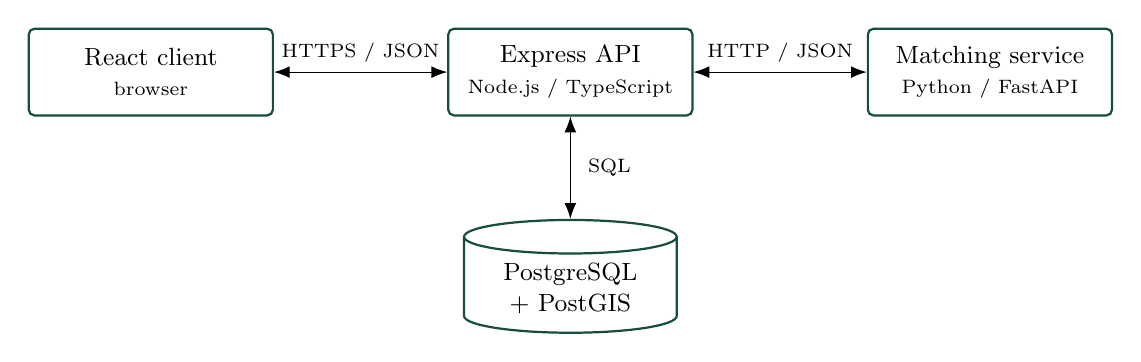
\begin{tikzpicture}[
  box/.style={draw=fbgreen!70!black, thick, rounded corners=2pt, align=center,
              minimum width=31mm, minimum height=11mm, font=\small},
  store/.style={draw=fbgreen!70!black, thick, cylinder, shape border rotate=90,
                aspect=0.22, align=center, minimum width=27mm,
                minimum height=13mm, font=\small},
  lbl/.style={font=\scriptsize, midway, sloped, above}
]
\node[box] (web) {React client\\\scriptsize browser};
\node[box, right=22mm of web] (api) {Express API\\\scriptsize Node.js / TypeScript};
\node[box, right=22mm of api] (match) {Matching service\\\scriptsize Python / FastAPI};
\node[store, below=13mm of api] (db) {PostgreSQL\\+ PostGIS};

\draw[{Latex[length=2mm]}-{Latex[length=2mm]}] (web) -- node[lbl]{HTTPS / JSON} (api);
\draw[{Latex[length=2mm]}-{Latex[length=2mm]}] (api) -- node[lbl]{HTTP / JSON} (match);
\draw[{Latex[length=2mm]}-{Latex[length=2mm]}] (api) -- node[font=\scriptsize,right=1mm]{SQL} (db);
\end{tikzpicture}
\caption{System architecture. The matching service holds no state; all
persistence is the API's responsibility.}
\end{figure}

\subsection{Product Functions}
\begin{itemize}
  \item Register and authenticate donors, recipient organisations and administrators.
  \item Accept a surplus food listing with quantity, type, location and expiry deadline.
  \item Allow an administrator to approve or reject each listing before it is matched.
  \item Filter organisations on hard constraints and rank the remainder on a weighted score.
  \item Offer a donation to the best-fit organisation and re-offer on decline or timeout.
  \item Record a two-stage pickup, confirmed by the collecting organisation.
  \item Notify both parties at every transition.
  \item Report impact metrics derived from system timestamps.
\end{itemize}

\subsection{User Classes and Characteristics}
\begin{description}[leftmargin=0pt,style=nextline,font=\normalfont\bfseries]
  \item[Donor \rm(\code{DONOR})]
    A mess hall, canteen, restaurant, caterer or event organiser. Technically
    unsophisticated, often submitting from a mobile device while clearing a
    kitchen. Interacts briefly and infrequently. The dominant class by volume of
    interactions; the submission form is designed around it.
  \item[Recipient Organisation \rm(\code{RECIPIENT})]
    A shelter, NGO, community kitchen, orphanage, old-age home or food bank.
    Represented by a coordinator who must answer an offer within a bounded
    window. Interacts more frequently than a donor and with more at stake, since
    an unanswered offer holds capacity.
  \item[Administrator \rm(\code{ADMIN})]
    A member of the operating team. Reviews every submitted donation, triggers
    matching cycles and monitors impact. Technically capable. Sits on the
    critical path: no donation is matched without an administrator.
\end{description}

\subsection{Stakeholders}
\begin{longtable}{@{}p{3.6cm}p{11cm}@{}}
\toprule
\textbf{Stakeholder} & \textbf{Interest in the system} \\
\midrule
\endhead
Donor organisations & Dispose of surplus responsibly with a record that it was collected; minimal effort per donation. \\
Recipient organisations & Source food at short notice matching their dietary constraints and capacity. \\
Beneficiaries & Indirect: receive redistributed meals. Not system users. \\
Operating team & Keep unsuitable listings out and see whether the system is working. \\
Development team & Deliver a correct, demonstrable and measurable system within the course timeline. \\
Course instructor & Assess engineering process, correctness and measurement against the proposal. \\
\bottomrule
\end{longtable}

\subsection{Operating Environment}
\begin{itemize}
  \item \textbf{Client:} any modern browser on desktop or mobile. No installation.
  \item \textbf{API:} Node.js 20 or later, Express, TypeScript.
  \item \textbf{Matching service:} Python 3.9 or later, FastAPI, SciPy, NumPy.
  \item \textbf{Database:} PostgreSQL 17 with the PostGIS 3.x spatial extension.
  \item \textbf{Network:} the three processes communicate over HTTP; only the
    client requires public reachability in deployment.
\end{itemize}

\subsection{Design and Implementation Constraints}
\begin{description}[leftmargin=1.9cm,style=nextline,font=\normalfont\bfseries]
  \item[CON-1] The interface must remain usable on low-to-mid range mobile
    devices. A donor's entire obligation must fit in one short form.
  \item[CON-2] Allocation must use classical, library-backed methods. No novel or
    learned algorithm may be introduced; the Hungarian method is consumed as a
    standard library primitive.
  \item[CON-3] The matching service must remain stateless and free of database
    dependencies, so it can be tested in isolation and replaced behind a fixed
    interface.
  \item[CON-4] Evaluation metrics must be derived from database timestamps
    written by the system, never from values entered by a user.
  \item[CON-5] Transport is arranged by the two matched parties. The system must
    not model vehicles, routes or drivers.
  \item[CON-6] Deployment must rely only on common web hosting, a managed
    relational database with a spatial extension, and free-tier external
    services.
  \item[CON-7] Geocoding must use a free-tier provider, and results must be
    cached to respect its rate limit of one request per second.
\end{description}

\subsection{Assumptions and Dependencies}
\begin{itemize}
  \item Both parties have a smartphone with intermittent internet access.
  \item An administrator is available to review submissions during operating
    hours. The consequence of this assumption for OBJ-2 is discussed in
    Section~5.1.
  \item Organisations declare their capacity, service radius and dietary
    constraints honestly; the system does not verify them independently.
  \item Food safety remains the donor's legal responsibility. Administrative
    review is a screening step, not a certification.
  \item The external geocoding provider remains available and free to use.
\end{itemize}

\section{External Interface Requirements}

\subsection{User Interfaces}
A responsive single-page web application. Navigation is role-aware: each user
class is shown only the screens belonging to it, and an attempt to reach another
class's screen is refused.

\begin{longtable}{@{}p{3.3cm}p{3.0cm}p{8.2cm}@{}}
\toprule
\textbf{Screen} & \textbf{User class} & \textbf{Purpose} \\
\midrule
\endhead
Sign in / Register & All & Authentication; registration branches by role. \\
Post donation & Donor & Single-screen submission form. \\
My donations & Donor & Listing with live countdowns; detail shows the status timeline. \\
Offers & Recipient & Pending offers with score breakdown and response countdown. \\
Collections & Recipient & Accepted donations; pickup confirmation. \\
Review queue & Administrator & Approve or reject submissions; trigger a matching cycle; view the waitlist. \\
Impact & Administrator & Metrics derived from system timestamps. \\
\bottomrule
\end{longtable}

\noindent
Minimum touch target 44\,px; every state change confirmed with visible feedback;
errors reported against the specific field that caused them.

\subsection{Hardware Interfaces}
None. The system requires no sensors, scanners or dedicated hardware. Location
is supplied as coordinates, or as a textual address resolved by the geocoding
service.

\subsection{Software Interfaces}
\begin{description}[leftmargin=0pt,style=nextline,font=\normalfont\bfseries]
  \item[PostgreSQL / PostGIS]
    Accessed over the Postgres wire protocol. Spatial predicates
    (\code{ST_DWithin}, \code{ST_Distance}) are evaluated in the database, so
    candidate retrieval does not degrade linearly with the number of registered
    organisations.
  \item[Matching service]
    A single operation, \code{POST /match/run}, accepting open donations,
    eligible organisations, precomputed pair distances and a configuration
    block; returning assignments, a waitlist and per-candidate explanations.
  \item[Geocoding provider]
    OpenStreetMap Nominatim over HTTPS, at most one request per second, with all
    results cached in \code{geocoding_cache}.
\end{description}

\subsection{Communications Interfaces}
All interfaces are JSON over HTTP. The client authenticates with a bearer token
obtained at sign-in and presented on every subsequent request. Errors use a
single envelope so the client can render any failure uniformly:

\begin{quote}
\code{{ "error": { "code": string, "message": string, "details"?: any } }}
\end{quote}

\noindent
HTTP status codes are used as specified: 400 validation, 401 authentication,
403 authorisation, 404 missing, 409 illegal state transition, 502 matching
service unreachable.

\section{System Features}

Figure~\ref{fig:usecase} shows the actors and their use cases. The functional
requirements that follow are grouped by feature.

\begin{landscape}
\begin{figure}[p]
\centering
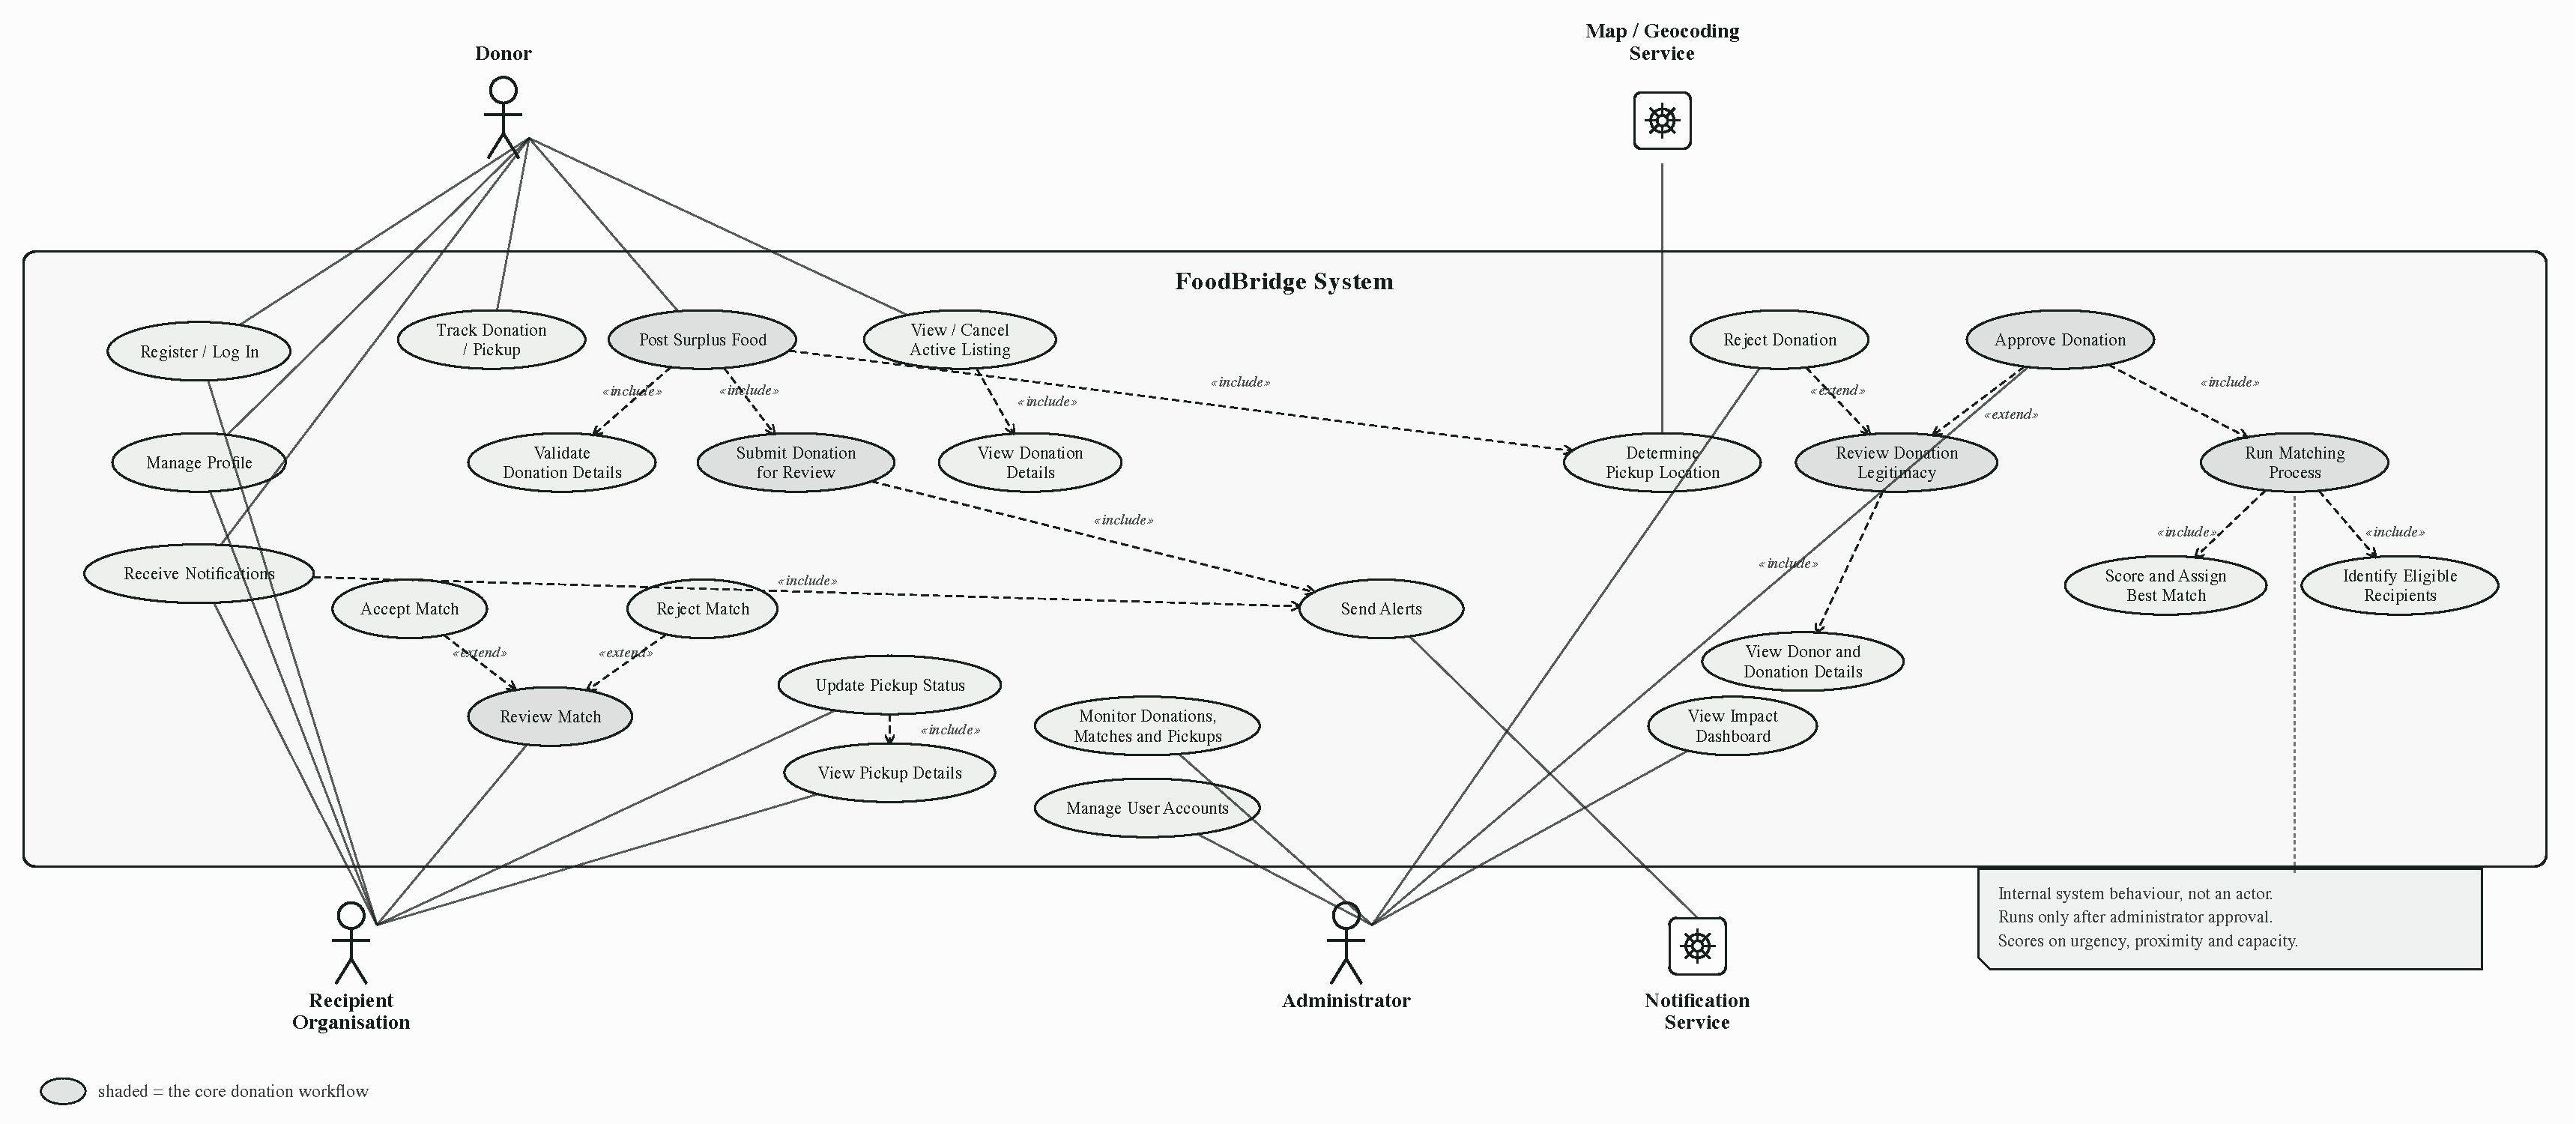
\includegraphics[width=\linewidth]{figures/use-case.pdf}
\caption{Use case diagram. Dashed arrows are stereotyped dependencies:
\emph{include} for behaviour the base use case always performs, \emph{extend}
for behaviour that occurs only under a condition.}
\label{fig:usecase}
\end{figure}
\end{landscape}

\noindent
Table~\ref{tab:uctrace} traces every use case in the figure to the requirements
that specify it, so that no element of the diagram is left unspecified and no
requirement is unmotivated.

\begingroup\small
\newcolumntype{L}[1]{>{\raggedright\arraybackslash}p{#1}}
\begin{longtable}{@{}L{6.0cm}L{4.5cm}L{4.4cm}@{}}
\caption{Use case to requirement traceability.}\label{tab:uctrace}\\
\toprule
\textbf{Use case} & \textbf{Feature (Section)} & \textbf{Requirements} \\
\midrule
\endfirsthead
\toprule
\textbf{Use case} & \textbf{Feature (Section)} & \textbf{Requirements} \\
\midrule
\endhead
\bottomrule
\endfoot
Register / Log In            & Account Management (4.1) & FR-1--FR-6 \\
Manage Profile               & Account Management (4.1) & FR-4, FR-7 \\
Post Surplus Food            & Donation Submission (4.2) & FR-8, FR-9 \\
Validate Donation Details    & Donation Submission (4.2) & FR-10 \\
Determine Pickup Location    & Donation Submission (4.2) & FR-11 \\
Submit Donation for Review   & Donation Submission (4.2) & FR-12, FR-13 \\
View / Cancel Active Listing & Donation Submission (4.2) & FR-14 \\
View Donation Details        & Donation Submission (4.2) & FR-15 \\
Track Donation / Pickup      & Donation Submission (4.2) & FR-15, FR-38 \\
Review Donation Legitimacy   & Administrative Review (4.3) & FR-16, FR-19, FR-20 \\
View Donor and Donation Details & Administrative Review (4.3) & FR-16 \\
Approve Donation             & Administrative Review (4.3) & FR-17, FR-21 \\
Reject Donation              & Administrative Review (4.3) & FR-18, FR-21 \\
Run Matching Process         & Matching and Allocation (4.4) & FR-26, FR-27, FR-31 \\
Identify Eligible Recipients & Matching and Allocation (4.4) & FR-22, FR-28, FR-30 \\
Score and Assign Best Match  & Matching and Allocation (4.4) & FR-23--FR-25, FR-29 \\
Review Match                 & Offer Response (4.5) & FR-32, FR-35 \\
Accept Match                 & Offer Response (4.5) & FR-33, FR-36, FR-37 \\
Reject Match                 & Offer Response (4.5) & FR-34, FR-36 \\
Update Pickup Status         & Pickup and Completion (4.6) & FR-39--FR-41 \\
View Pickup Details          & Pickup and Completion (4.6) & FR-38 \\
Send Alerts                  & Notification (4.7) & FR-42, FR-44 \\
Receive Notifications        & Notification (4.7) & FR-43 \\
View Impact Dashboard        & Impact Reporting (4.8) & FR-45--FR-49 \\
Monitor Donations, Matches and Pickups & Administrative Oversight (4.11) & FR-54 \textit{(deferred)} \\
Manage User Accounts         & Administrative Oversight (4.11) & FR-55 \textit{(deferred)} \\
\end{longtable}
\endgroup

\noindent
The last two rows are the only use cases in the diagram that release~1.0 does
not implement; they are specified in Section~4.11 and marked deferred rather
than removed from the diagram, so that the team's agreed scope and the
delivered scope can be compared directly.

\subsection{Account Management and Authentication}
\textbf{Priority: Essential.} Every interaction other than registration and
sign-in requires an authenticated principal whose role determines what is
permitted.

\begin{description}[leftmargin=1.6cm,style=nextline,font=\normalfont\bfseries]
  \req{FR-1}{The system shall allow a visitor to register as a donor or as a
    recipient organisation, capturing name, e-mail, password and role.}
  \req{FR-2}{The system shall reject a password shorter than eight characters.}
  \req{FR-3}{The system shall store passwords only as a one-way hash; no
    plaintext password shall be persisted or logged.}
  \req{FR-4}{The system shall capture, for a recipient organisation, its
    organisation type, serving capacity, service radius in kilometres, accepted
    food types, dietary restrictions and location.}
  \req{FR-5}{The system shall issue a time-limited bearer token at successful
    sign-in and reject an expired or malformed token with HTTP 401.}
  \req{FR-6}{The system shall derive the caller's role from the token and refuse,
    with HTTP 403, any request to an operation that role does not permit.}
  \req{FR-7}{The system shall allow an authenticated user to retrieve and update
    their own profile, including an organisation's capacity, radius, preferences
    and active flag.}
\end{description}

\subsection{Donation Submission}
\textbf{Priority: Essential.} The donor's entire obligation.

\begin{description}[leftmargin=1.6cm,style=nextline,font=\normalfont\bfseries]
  \req{FR-8}{The system shall allow a donor to submit a donation specifying food
    type, quantity in whole servings, pickup location and an expiry deadline.}
  \req{FR-9}{The system shall accept the expiry deadline either as an absolute
    timestamp or as a number of hours from submission.}
  \req{FR-10}{The system shall reject a submission whose quantity is not a
    positive whole number, or whose deadline is not in the future, reporting the
    offending field.}
  \req{FR-11}{The system shall resolve the pickup location server-side: explicit
    coordinates are used as given; otherwise a textual address is resolved
    through the geocoding cache and then, on a miss, the external provider.}
  \req{FR-12}{The system shall assign every new donation the status
    \code{PENDING_REVIEW} and record its submission timestamp.}
  \req{FR-13}{The system shall notify all administrators that a submission
    awaits review.}
  \req{FR-14}{The system shall allow a donor to cancel their own donation while
    it is \code{PENDING_REVIEW} or \code{POSTED}, and not afterwards.}
  \req{FR-15}{The system shall allow a donor to view their own donations and the
    full history of any one of them, and shall refuse access to another donor's
    donation.}
\end{description}

\subsection{Administrative Review}
\textbf{Priority: Essential.} No donation reaches an organisation without an
approval, which is the system's screening control for listing quality and food
safety.

\begin{description}[leftmargin=1.6cm,style=nextline,font=\normalfont\bfseries]
  \req{FR-16}{The system shall present administrators with a queue of all
    donations in \code{PENDING_REVIEW}.}
  \req{FR-17}{The system shall allow an administrator to approve a donation,
    moving it to \code{POSTED} and making it eligible for matching.}
  \req{FR-18}{The system shall allow an administrator to reject a donation with
    recorded remarks, moving it to \code{REJECTED}.}
  \req{FR-19}{The system shall persist every review decision, its author and its
    timestamp, as an audit record that survives subsequent decisions.}
  \req{FR-20}{The system shall refuse a second review of an already-reviewed
    donation with HTTP 409.}
  \req{FR-21}{The system shall notify the donor of the review outcome.}
\end{description}

\subsection{Matching and Allocation}
\textbf{Priority: Essential.} The system's reason for existing, and the
component OBJ-3 isolates behind a service boundary.

\begin{description}[leftmargin=1.6cm,style=nextline,font=\normalfont\bfseries]
  \req{FR-22}{The system shall exclude from consideration, before any scoring,
    any organisation that is inactive, lacks sufficient remaining capacity for
    the donation, does not accept the donation's food type, or lies outside the
    current search radius.}
  \req{FR-23}{The system shall compute, for every surviving organisation, a
    weighted score over three normalised components --- urgency (0.40),
    proximity (0.35) and capacity fit (0.25).}
  \req{FR-24}{The system shall treat the component weights as configuration
    rather than as embedded logic.}
  \req{FR-25}{The system shall persist, with every offer, its total score and
    each component score, so that any allocation can be explained after the
    fact.}
  \req{FR-26}{The system shall support two allocation strategies --- a greedy
    best-fit assignment and a global assignment using the Hungarian method ---
    selectable per matching cycle.}
  \req{FR-27}{The system shall begin matching at a search radius of 5\,km and
    widen it in 5\,km steps to a maximum of 25\,km when no organisation is
    eligible.}
  \req{FR-28}{The system shall place on a waitlist, rather than discard, any
    donation for which no organisation is eligible at the maximum radius, and
    shall retry it on each subsequent cycle, recording the number of attempts.}
  \req{FR-29}{The system shall reserve an organisation's capacity for the
    duration of an outstanding offer, so that the same capacity cannot be
    promised to two donations simultaneously.}
  \req{FR-30}{The system shall return a per-candidate explanation for every
    donation processed, stating for each organisation whether it was eligible
    and, if not, which constraint excluded it.}
  \req{FR-31}{The system shall report an unreachable matching service as
    HTTP 502 and shall not alter donation state in that event.}
\end{description}

\subsection{Offer Response}
\textbf{Priority: Essential.}

\begin{description}[leftmargin=1.6cm,style=nextline,font=\normalfont\bfseries]
  \req{FR-32}{The system shall present to a recipient organisation only those
    offers directed at it.}
  \req{FR-33}{The system shall allow an organisation to accept an offer, moving
    the offer to \code{ACCEPTED} and creating a scheduled pickup.}
  \req{FR-34}{The system shall allow an organisation to reject an offer, moving
    the donation back to \code{POSTED}, excluding that organisation from the
    immediate retry, and running a fresh matching cycle.}
  \req{FR-35}{The system shall expire an offer unanswered after its response
    window of 30 minutes, release the capacity it reserved, and return the
    donation for re-matching.}
  \req{FR-36}{The system shall refuse a response to an offer that has already
    been answered or has expired, with HTTP 409.}
  \req{FR-37}{The system shall disclose the counterparty's contact details only
    after an offer has been accepted.}
\end{description}

\subsection{Pickup and Completion}
\textbf{Priority: Essential.}

\begin{description}[leftmargin=1.6cm,style=nextline,font=\normalfont\bfseries]
  \req{FR-38}{The system shall create a pickup record in \code{SCHEDULED} when an
    offer is accepted, carrying the scheduled time and the contact details.}
  \req{FR-39}{The system shall allow the collecting organisation to record
    collection, moving the pickup to \code{PICKED_UP} and the donation to
    \code{PICKED_UP} in one transaction.}
  \req{FR-40}{The system shall allow the collecting organisation to confirm
    receipt, moving the pickup and the donation to \code{COMPLETED} and
    releasing the organisation's reserved capacity, in one transaction.}
  \req{FR-41}{The system shall refuse any transition not permitted from the
    current state, with HTTP 409 and without partial effect.}
\end{description}

\subsection{Notification}
\textbf{Priority: Essential for the workflow; the channel is in-app only in
release~1.0.}

\begin{description}[leftmargin=1.6cm,style=nextline,font=\normalfont\bfseries]
  \req{FR-42}{The system shall raise an in-app notification to the affected
    parties at every state transition of a donation, offer or pickup.}
  \req{FR-43}{The system shall report an unread count and allow a user to mark
    one notification, or all of them, as read.}
  \req{FR-44}{The system shall deliver notification by e-mail or SMS.
    \textit{(Deferred.)}}
\end{description}

\subsection{Impact Reporting}
\textbf{Priority: Essential.} The mechanism by which OBJ-2 is evaluated.

\begin{description}[leftmargin=1.6cm,style=nextline,font=\normalfont\bfseries]
  \req{FR-45}{The system shall compute and report servings redistributed,
    completed donations, donations lost to expiry, the unmatched rate, the
    waitlist size and waste diverted.}
  \req{FR-46}{The system shall compute median and mean time-to-match from the
    interval between a donation's submission timestamp and the response
    timestamp of its first accepted offer.}
  \req{FR-47}{The system shall compute every reported metric server-side from
    persisted timestamps; the client shall not derive any metric.}
  \req{FR-48}{The system shall report the first-offer acceptance rate and the
    mean donor-to-recipient distance. \textit{(Deferred.)}}
  \req{FR-49}{The system shall collect a 1--5 clarity rating of the status
    timeline from both parties after completion. \textit{(Deferred.)}}
\end{description}

\subsection{Organisation Verification}
\textbf{Priority: Deferred.} In release~1.0 legitimacy is screened per donation
(Section~4.3) rather than per organisation.

\begin{description}[leftmargin=1.6cm,style=nextline,font=\normalfont\bfseries]
  \req{FR-50}{The system shall allow a recipient organisation to upload
    registration documents and shall record a verification status of
    \code{PENDING}, \code{APPROVED} or \code{REJECTED}. \textit{(Deferred.)}}
  \req{FR-51}{The system shall exclude an unverified organisation from matching.
    \textit{(Deferred.)}}
\end{description}

\subsection{Unattended Operation}
\textbf{Priority: Deferred, and the highest-priority item for the next
iteration.} In release~1.0 expiry and re-matching occur only when an
administrator triggers a cycle.

\begin{description}[leftmargin=1.6cm,style=nextline,font=\normalfont\bfseries]
  \req{FR-52}{The system shall expire overdue donations and offers automatically
    on a schedule, without administrator action. \textit{(Deferred.)}}
  \req{FR-53}{The system shall surface a manual list of nearby organisations to
    the donor when automated matching finds none. \textit{(Deferred.)}}
\end{description}

\subsection{Administrative Oversight}
\textbf{Priority: Deferred.} In release~1.0 an administrator's view of the
system is limited to the pending-review queue and the matching waitlist; there
is no global listing of donations, matches and pickups and no account
administration beyond a user's own profile.

\begin{description}[leftmargin=1.6cm,style=nextline,font=\normalfont\bfseries]
  \req{FR-54}{The system shall present an administrator with a filterable view
    of all donations, offers and pickups across every user, independent of
    review state. \textit{(Deferred.)}}
  \req{FR-55}{The system shall allow an administrator to deactivate, reactivate
    or change the role of a user account, and shall record the acting
    administrator and the time of each such change. \textit{(Deferred.)}}
\end{description}

\section{Other Nonfunctional Requirements}

\subsection{Performance Requirements}
\begin{description}[leftmargin=1.9cm,style=nextline,font=\normalfont\bfseries]
  \req{NFR-1}{The median time-to-match shall be 20 minutes or less during the
    pilot window (OBJ-2).}
  \req{NFR-2}{Candidate retrieval shall use a spatial index so that it does not
    degrade linearly with the number of registered organisations.}
  \req{NFR-3}{A matching cycle over the pilot dataset shall complete within
    5~seconds.}
  \req{NFR-4}{An interactive request shall complete within 2~seconds under pilot
    load.}
  \req{NFR-5}{The client shall remain usable on a low-to-mid range mobile device
    over a mobile data connection.}
\end{description}

\noindent\textbf{Note on NFR-1.} The implemented workflow places an
administrative review between submission and matching, so the measured interval
includes administrator response time. The pilot must therefore either record
review latency separately or measure from approval rather than from submission,
and must state which definition it uses. This is recorded as TBD-1 in
Appendix~C.

\subsection{Safety Requirements}
\begin{description}[leftmargin=1.9cm,style=nextline,font=\normalfont\bfseries]
  \req{NFR-6}{No donation shall be matched before an administrator has approved
    it.}
  \req{NFR-7}{The system shall not assign a donation to an organisation whose
    declared dietary constraints exclude its food type.}
  \req{NFR-8}{The system shall not promise the same capacity to two donations
    simultaneously.}
  \req{NFR-9}{A donation reaching its deadline uncollected shall be recorded as
    expired and counted against the system's own performance, not silently
    discarded.}
\end{description}

\subsection{Security Requirements}
\begin{description}[leftmargin=1.9cm,style=nextline,font=\normalfont\bfseries]
  \req{NFR-10}{All passwords shall be stored as one-way hashes using an adaptive
    hashing function.}
  \req{NFR-11}{Authorisation shall be enforced at the server for every
    operation; the client shall not be treated as a security boundary.}
  \req{NFR-12}{A user shall be able to read and modify only their own resources,
    except an administrator acting within their defined operations.}
  \req{NFR-13}{Personal contact details shall be disclosed only after an offer
    has been accepted.}
  \req{NFR-14}{Collected personal data shall be minimised to what the workflow
    requires.}
  \req{NFR-15}{The production deployment shall not use a development signing
    secret.}
\end{description}

\subsection{Software Quality Attributes}
\begin{description}[leftmargin=1.9cm,style=nextline,font=\normalfont\bfseries]
  \req{NFR-16}{\textbf{Testability.} The matching service shall be testable in
    isolation, taking all state as input and returning a result, with no
    database dependency.}
  \req{NFR-17}{\textbf{Explainability.} Every allocation shall be reconstructable
    after the fact from stored score components and recorded exclusion reasons.}
  \req{NFR-18}{\textbf{Modifiability.} The allocation strategy shall be
    replaceable without modification to the API or the client.}
  \req{NFR-19}{\textbf{Auditability.} Every state transition shall be persisted
    with its timestamp and its actor.}
  \req{NFR-20}{\textbf{Usability.} A donor shall be able to complete a submission
    on one screen without scrolling past a single form.}
  \req{NFR-21}{\textbf{Reliability.} Staging and production availability shall be
    99\% or better during the pilot window.}
  \req{NFR-22}{\textbf{Interoperability.} The API contract shall be verifiable by
    an automated conformance check that fails the build on any breach.}
\end{description}

\subsection{Business Rules}
\begin{description}[leftmargin=1.9cm,style=nextline,font=\normalfont\bfseries]
  \req{BR-1}{Only an administrator may approve or reject a donation.}
  \req{BR-2}{Only the owning donor may cancel a donation, and only before
    collection.}
  \req{BR-3}{Only the organisation an offer was made to may accept or reject it.}
  \req{BR-4}{Only the collecting organisation may record collection and confirm
    receipt.}
  \req{BR-5}{Acceptance is a property of an offer, not of a donation. A donation
    may be offered to several organisations in sequence.}
  \req{BR-6}{An organisation that rejects an offer is excluded from the
    immediate retry for that donation.}
  \req{BR-7}{A donation is never discarded for want of an eligible organisation;
    it is waitlisted and retried.}
\end{description}

\section{Other Requirements}

\subsection{Database Requirements}
Persistence uses a relational database with a spatial extension. Locations are
stored as geography points under SRID~4326 with GiST indexes, so that
radius-constrained retrieval is evaluated in the query rather than in
application code. The schema comprises ten tables: users, donors, recipient
organisations, donations, matches, pickups, donation reviews, the matching
waitlist, notifications and the geocoding cache.

\subsection{Internationalisation}
Release~1.0 is English-only, with distances in kilometres, quantities in
servings and timestamps displayed in the viewer's local timezone. Multilingual
support is out of scope.

\appendix
\section{Glossary}
\begin{longtable}{@{}p{3.8cm}p{10.8cm}@{}}
\toprule
\textbf{Term} & \textbf{Definition} \\
\midrule
\endhead
Donation & A listing of surplus food offered by a donor. \\
Match / Offer & A proposal of one donation to one organisation, carrying its scores and a response deadline. \\
Pickup & The record of a physical handover, with its own lifecycle. \\
Time-to-Match & Interval between a donation's submission and the response time of its first accepted offer. \\
Rescue rate & Proportion of posted donations reaching \code{COMPLETED} before their deadline. \\
Waitlist & Donations for which no organisation was eligible, retained for retry. \\
Capacity fit & Normalised measure of how well a donation's size suits an organisation's remaining capacity. \\
Urgency & Normalised measure of how little time remains before a donation expires. \\
Greedy assignment & Strategy processing donations in urgency order, committing each to its best available organisation. \\
Hungarian method & Classical algorithm solving the one-to-one assignment problem optimally over all open donations. \\
PostGIS & Spatial extension to PostgreSQL providing geography types and spatial indexes. \\
\bottomrule
\end{longtable}

\section{Analysis Models}

\subsection{Donation State Machine}
Figure~\ref{fig:states} shows the permitted transitions. Each is validated
centrally; an illegal transition is refused with HTTP 409 and has no partial
effect. Acceptance does not appear as a donation state: it is a property of the
offer (BR-5).

\begin{figure}[h]
\centering
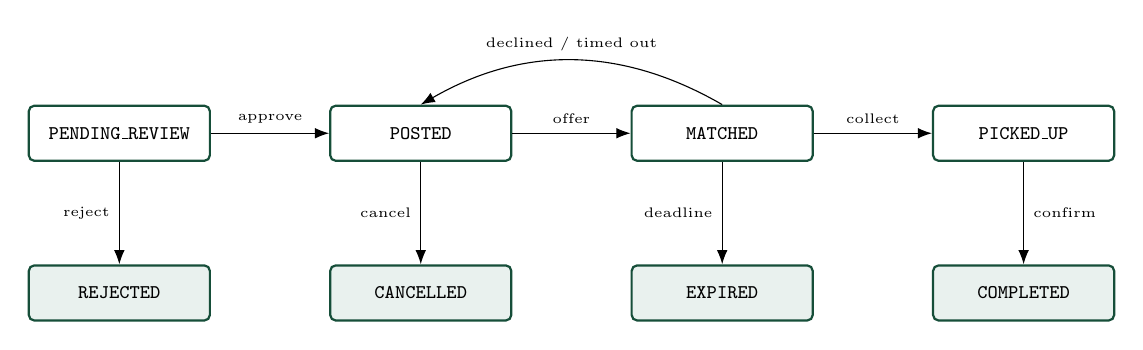
\begin{tikzpicture}[
  node distance=13mm and 15mm,
  st/.style={draw=fbgreen!70!black, thick, rounded corners=2pt,
             font=\scriptsize\ttfamily, minimum height=7mm,
             minimum width=23mm, align=center},
  term/.style={st, fill=fbgreen!10},
  ar/.style={-{Latex[length=1.8mm]}, thin},
  lb/.style={font=\tiny, midway}
]
\node[st] (pr) {PENDING\_REVIEW};
\node[st, right=of pr] (po) {POSTED};
\node[st, right=of po] (ma) {MATCHED};
\node[st, right=of ma] (pu) {PICKED\_UP};
\node[term, below=of pu] (co) {COMPLETED};
\node[term, below=of pr] (rj) {REJECTED};
\node[term, below=of po] (ca) {CANCELLED};
\node[term, below=of ma] (ex) {EXPIRED};

\draw[ar] (pr) -- node[lb,above]{approve} (po);
\draw[ar] (po) -- node[lb,above]{offer} (ma);
\draw[ar] (ma) -- node[lb,above]{collect} (pu);
\draw[ar] (pu) -- node[lb,right]{confirm} (co);
\draw[ar] (pr) -- node[lb,left]{reject} (rj);
\draw[ar] (po) -- node[lb,left]{cancel} (ca);
\draw[ar] (ma) -- node[lb,left]{deadline} (ex);
\draw[ar] (ma.north) to[bend right=30] node[lb,above]{declined / timed out} (po.north);
\end{tikzpicture}
\caption{Donation lifecycle. The curved return from \code{MATCHED} to
\code{POSTED} is the re-match path (FR-34, FR-35).}
\label{fig:states}
\end{figure}

\subsection{Matching Pipeline}
\begin{figure}[h]
\centering
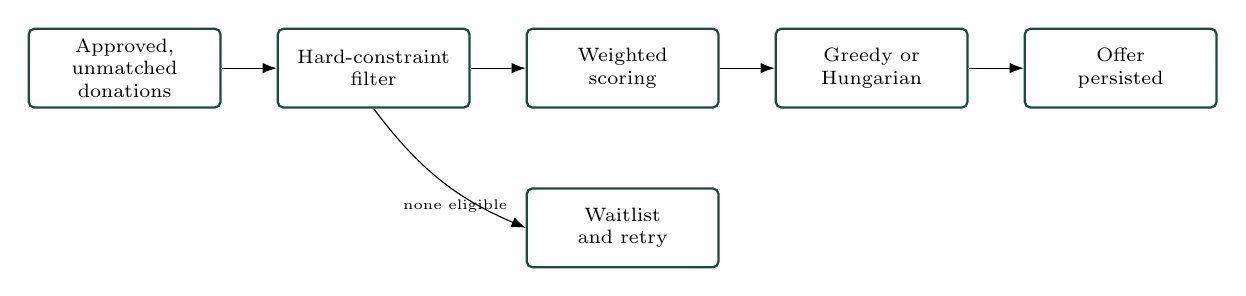
\begin{tikzpicture}[
  node distance=7mm,
  stg/.style={draw=fbgreen!70!black, thick, rounded corners=2pt, font=\scriptsize,
              minimum height=10mm, text width=22mm, align=center},
  ar/.style={-{Latex[length=1.8mm]}, thin}
]
\node[stg] (a) {Approved,\\unmatched\\donations};
\node[stg, right=of a] (b) {Hard-constraint\\filter};
\node[stg, right=of b] (c) {Weighted\\scoring};
\node[stg, right=of c] (d) {Greedy or\\Hungarian};
\node[stg, right=of d] (e) {Offer\\persisted};
\node[stg, below=10mm of c] (w) {Waitlist\\and retry};
\foreach \x/\y in {a/b, b/c, c/d, d/e} \draw[ar] (\x) -- (\y);
\draw[ar] (b.south) to[bend right=15] node[font=\tiny,below,pos=0.6]{none eligible} (w.west);
\end{tikzpicture}
\caption{Filter, then rank. Eligibility is settled before any scoring, so an
organisation failing a hard constraint never competes on score (FR-22).}
\end{figure}

\section{Open Issues}
\begin{longtable}{@{}p{1.6cm}p{13cm}@{}}
\toprule
\textbf{ID} & \textbf{Issue} \\
\midrule
\endhead
TBD-1 & Whether time-to-match is measured from submission or from administrative approval. Affects NFR-1 and the pilot's baseline comparison. \\
TBD-2 & Whether a fairness term damping repeat allocation to the same organisation is added as a fourth scoring component. \\
TBD-3 & The response window of 30 minutes is provisional and should be calibrated against observed organisation response times during the pilot. \\
TBD-4 & Whether organisation verification (FR-50, FR-51) replaces or supplements per-donation review. \\
\bottomrule
\end{longtable}

\end{document}
